\subsubsection{An\'alise Explorat\'oria dos Dados (EDA)}

A partir do passo \ref{etp:1}, foi realizado o EDA (do inglês \textit{Exploratory Data Analysis}) para processar os dados obtidos até o momento. O EDA permite responder às questões de pesquisa levantadas. Conforme mencionado por \citeonline{Yu2016}, na era do \textit{big data}, é desafiador descobrir as regras, modelos analíticos e hipóteses por trás dos volumes massivos de dados caóticos, não estruturados e multimídia coletados por meio de vários canais. A análise exploratória de dados foi promovida por John Tukey como uma abordagem para explorar os dados, resumir suas principais características e formular hipóteses que possam direcionar a coleta adicional de dados e experimentos. No contexto de análises de dados, várias técnicas de EDA têm sido adotadas.

Na Figura \ref{fig:person} que ambas as variáveis apresentam uma correlação quase perfeita, com um coeficiente de correlação de Pearson ($r$) igual a $1$. Portanto, para responder a essa pergunta, basta observar a correlação de Pearson na Figura \ref{fig:person}. Na análise de correlação de Pearson, todo o conjunto de dados da SANEPAR foi utilizado para que cada variável pudesse ser avaliada quanto à sua correlação com a variável LT01. Se houvesse correlação, a variável era usada como variável exógena para melhorar os modelos. Como o modelo de LR consegue relacionar apenas uma ou duas variáveis entre si, no modelo de LR, LT01 foi usada como variável independente e PT01 como variável dependente.

\begin{figure}[H]
	\centering
	\caption{Correlação de Pearson}
	\label{fig:person}
	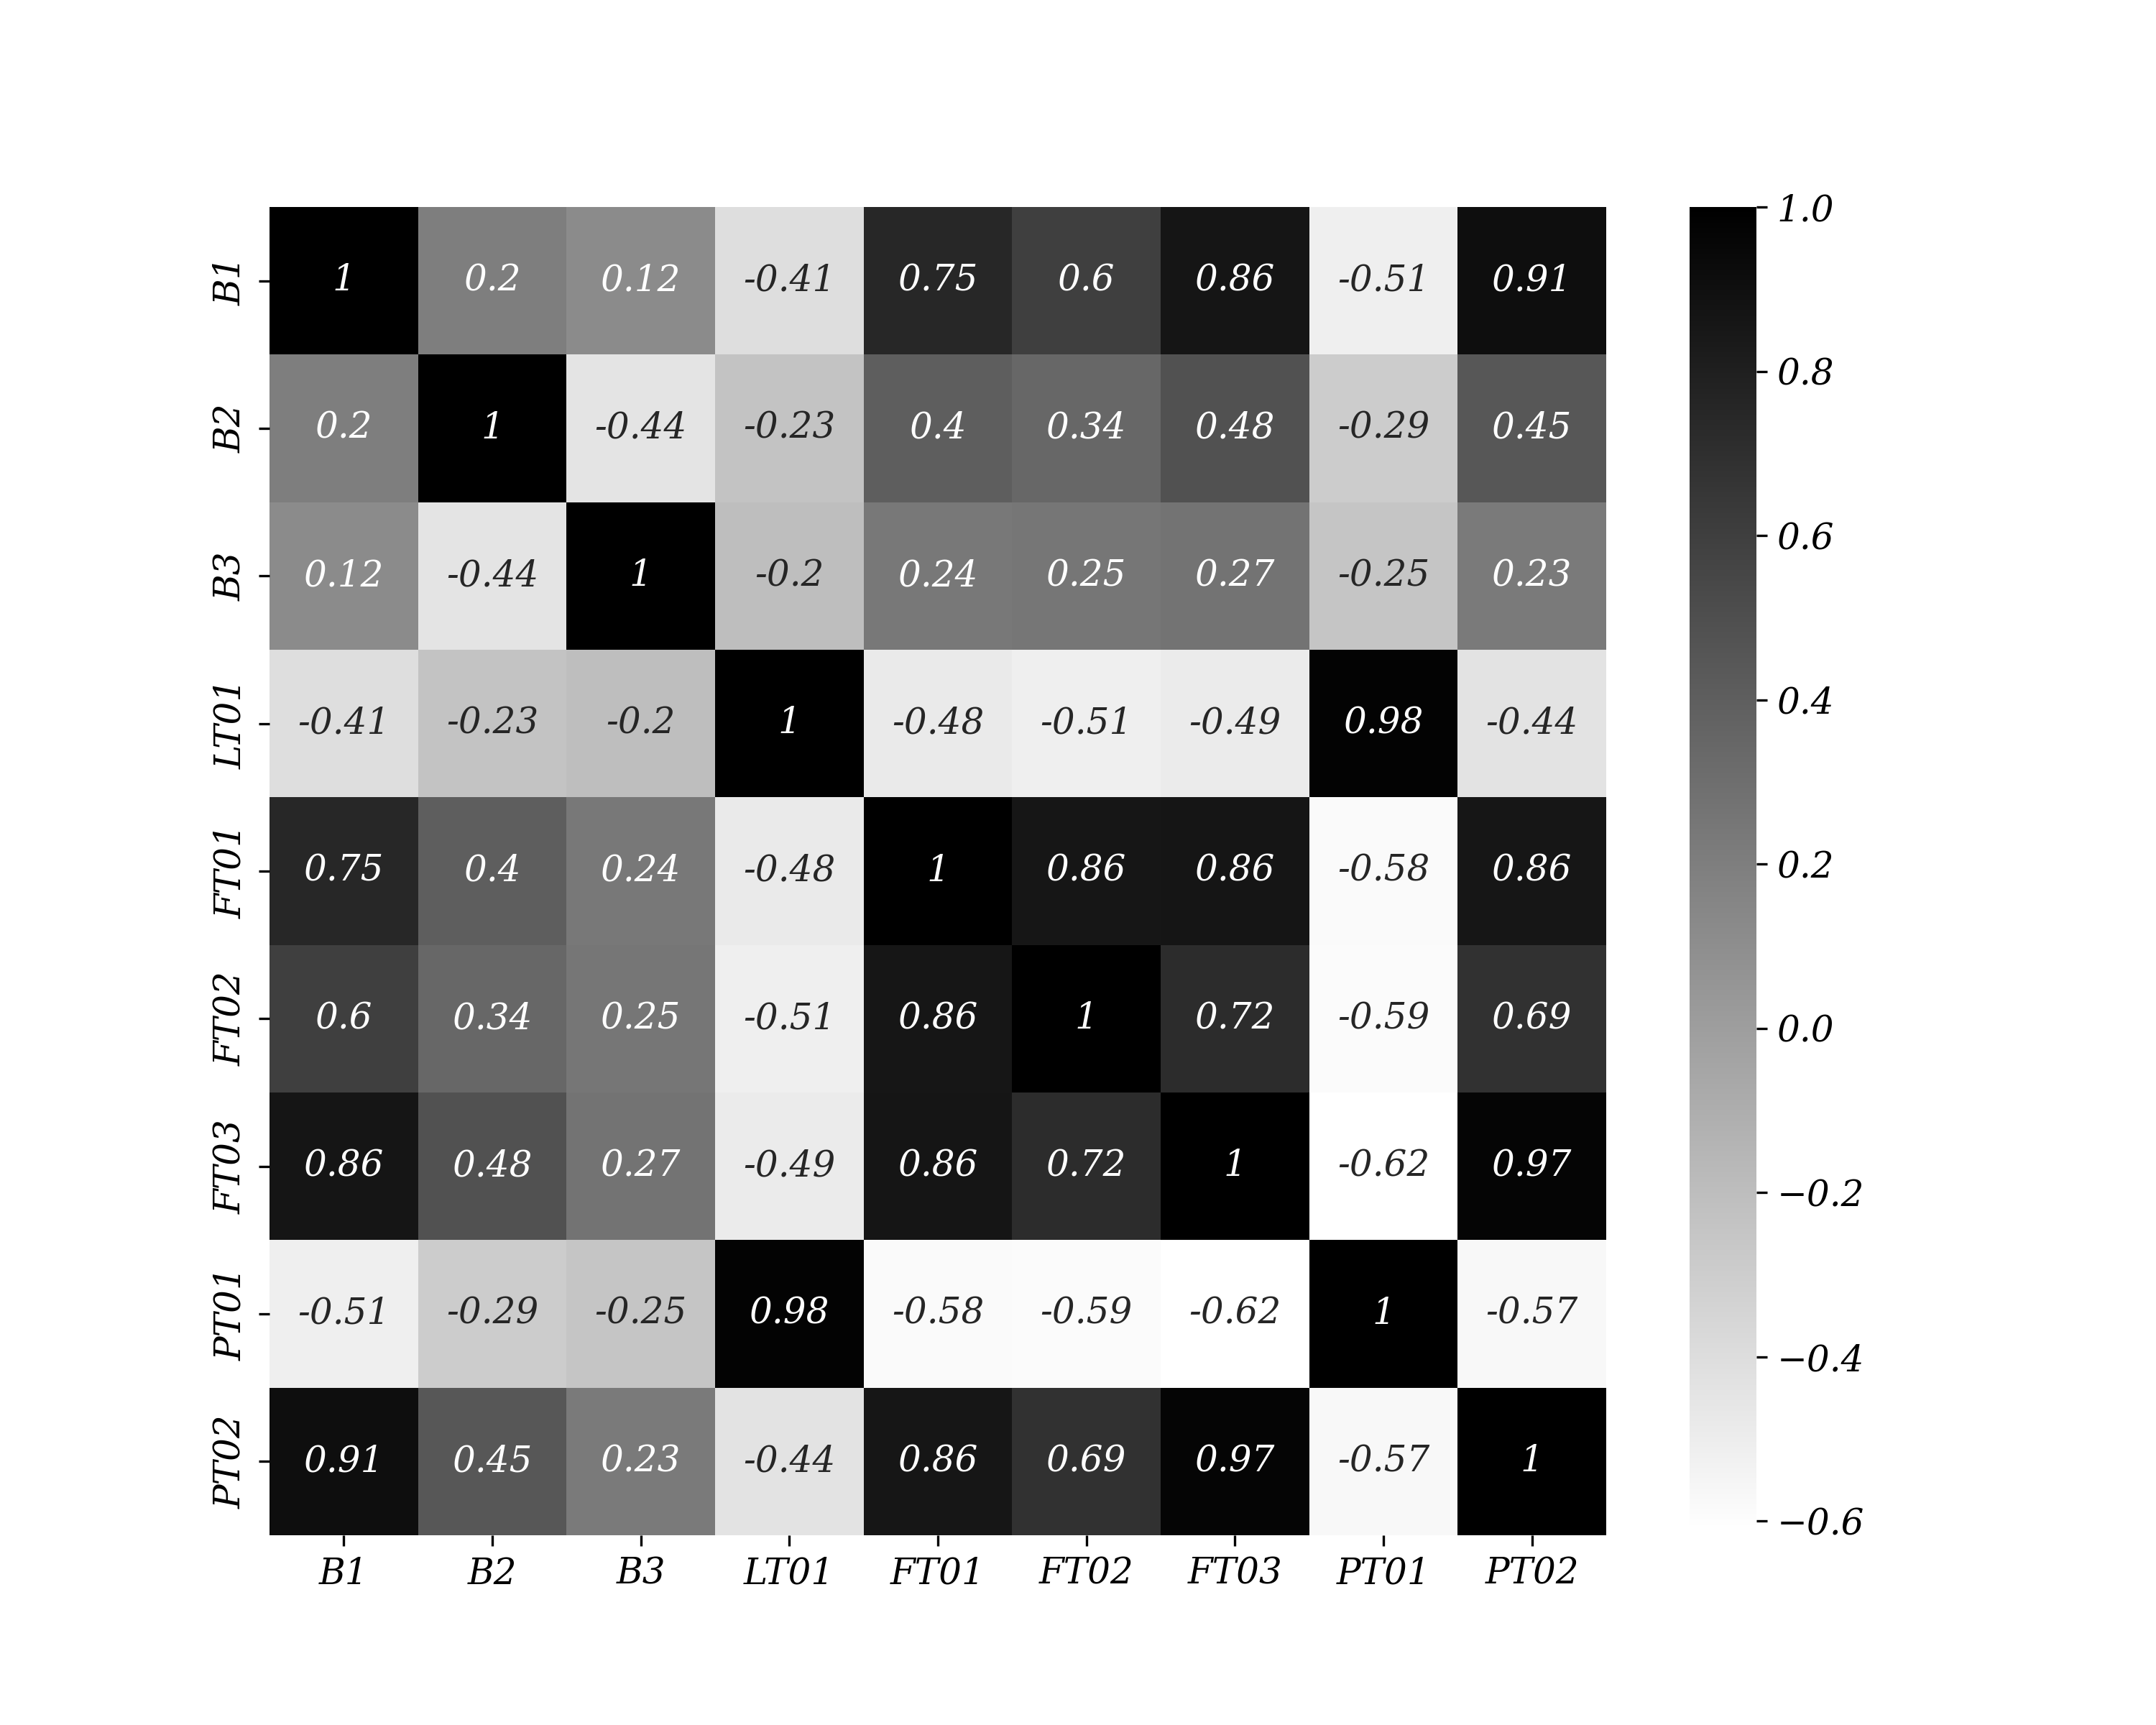
\includegraphics[width=0.9\linewidth]{Apendices/Figuras/modelagem-24h/person}
	
	
\end{figure}

A Figura \ref{fig:person} ilustra a correlação entre as variáveis no conjunto de dados em questão. Essa imagem representa graficamente a relação entre as variáveis e é usada para evidenciar a existência de uma correlação forte no valor de $0,98$ é considerada forte entre elas, quanto mais próximo do valor $1$ a correlação é sempre forte e $0,9$ para mais ou para menos indica uma correlação muito forte, 0 a $0,3$ positivo ou negativo indica uma correlação desprezível.


Na Tabela \ref{tb:est}, o desvio padrão é representado pela sigla STD, que corresponde à expressão em inglês \textit{standard deviation}. Além disso, em resposta à pergunta \ref{q2}, é importante mencionar que, assim como em qualquer empresa de tratamento de água, é utilizado um mecanismo de acionamento automático denominado ``trava de segurança'' para evitar que o nível do tanque se aproxime de zero e haja falta de água nos locais abastecidos por esse tanque. O nível mínimo que o tanque pode alcançar é de $5,29 m^3$ (equivalente a $5.285,90$ litros). As bombas são ativadas em sua potência máxima para evitar que sejam acionadas quando o nível do tanque. No entanto, a bomba $1$ ainda estaria operando para completar o nível do tanque caso ele esteja dentro dessa faixa.

\begin{table}[H]
	\centering
	\caption{Descrição estatística dos dados com o filtro aplicado das 18h às 21h}\label{tb:est}
	\begin{tabular}{@{}cccccccccc@{}}
		\toprule
		\textbf{18 a 21h}  & \textbf{B1} & \textbf{B2} & \textbf{B3} & \textbf{LT01} & \textbf{FT01} & \textbf{FT02} & \textbf{FT03} & \textbf{PT01} & \textbf{PT02} \\ \midrule
		\textbf{Contagem} & 4385    & 4385     & 4385     & 4385      & 4385       & 4385       & 4385       & 4385       & 4385       \\
		\textbf{Média}      & 51,94       & 27,81       & 6,41        & 3,24          & 112,68        & 132,93        & 112,41        & 4,11          & 20,80         \\
		\textbf{STD}       & 17,14       & 17,61       & 16,77       & 0,70          & 132,59        & 44,78         & 31,33         & 0,76          & 6,14          \\
		\textbf{Min}       & 0           & 0           & 0           & 0,29          & 0             & 0             & 0             & 0,88          & 0             \\
		\textbf{25\%}      & 57,84       & 0           & 0           & 2,79          & 0,12          & 123,96        & 111,66        & 3,62          & 21,72         \\
		\textbf{50\%}      & 57,99       & 34,91       & 0           & 3,30          & 0,12          & 136,00        & 118,82        & 4,15          & 22,05         \\
		\textbf{75\%}      & 57,99       & 38,02       & 0           & 3,78          & 264,27        & 148,20        & 125,63        & 4,66          & 23,02         \\
		\textbf{Max}       & 59,99       & 59,99       & 59,99       & 4,40          & 383,87        & 326,17        & 194,35        & 5,68          & 28,08         \\ \bottomrule
	\end{tabular}
	
	
\end{table}





Em situações de demanda de pico, uma abordagem ideal, embora não necessariamente a mais econômica, seria ter um tanque de reserva adicional e instalar uma tubulação que os conecte. Durante o dia, ambos os tanques seriam abastecidos e, à noite, por meio da ação da gravidade, eles manteriam o mesmo nível até que o consumo atinja um ponto em que as bombas sejam acionadas. Essa estratégia permite um abastecimento contínuo de água.


